\documentclass[a4paper]{article}

\usepackage{INTERSPEECH2016}

\usepackage{graphicx}
\usepackage{amssymb,amsmath,bm}
\usepackage{textcomp}
\usepackage{algorithm}
\usepackage{algpseudocode}

% Custom settings
\usepackage{tikz,placeins}
\tikzstyle{every picture}+=[font=\rmfamily\it\bfseries\large]

\graphicspath{{../figures/}}
% End of custom settings

\usepackage[tight,footnotesize]{subfigure}

\def\vec#1{\ensuremath{\bm{{#1}}}}
\def\mat#1{\vec{#1}}

\newcommand{\specialcell}[2][c]{%
   \begin{tabular}[#1]{@{}c@{}}#2\end{tabular}}


\newcommand{\chanwcom}{{C. Kim}}
\renewcommand{\topfraction}{1.0}
\renewcommand{\bottomfraction}{1.0}
\renewcommand{\textfraction}{0.01}
\renewcommand{\floatpagefraction}{1.0}
\renewcommand{\dbltopfraction}{1.0}
\renewcommand{\floatpagefraction}{1.0}  % require fuller float pages
\renewcommand{\dblfloatpagefraction}{1.0} % require fuller float pages


\sloppy % better line breaks
\ninept

\title{Phase distortion model for training phase-sensitive deep-neural networks for far-field speech recognition}

%%%%%%%%%%%%%%%%%%%%%%%%%%%%%%%%%%%%%%%%%%%%%%%%%%%%%%%%%%%%%%%%%%%%%%%%%%
%% If multiple authors, uncomment and edit the lines shown below.       %%
%% Note that each line must be emphasized {\em } by itself.             %%
%% (by Stephen Martucci, author of spconf.sty).                         %%
%%%%%%%%%%%%%%%%%%%%%%%%%%%%%%%%%%%%%%%%%%%%%%%%%%%%%%%%%%%%%%%%%%%%%%%%%%
%\makeatletter
%\def\name#1{\gdef\@name{#1\\}}
%\makeatother
%\name{{\em Firstname1 Lastname1, Firstname2 Lastname2, Firstname3 Lastname3,}\\
%      {\em Firstname4 Lastname4, Firstname5 Lastname5, Firstname6 Lastname6,
%      Firstname7 Lastname7}}
%%%%%%%%%%%%%%% End of required multiple authors changes %%%%%%%%%%%%%%%%%

\makeatletter
\def\name#1{\gdef\@name{#1\\}}
\makeatother \name{{\em Chanwoo Kim$^1$, Taran Sainath$^1$, Arun Narayana$^1$} \\ { \em Ananya Misra$^1$,
Rajeev Nongpiur$^2$, and Michiel Bacchiani$^1$}}


\address{$^1$Google Speech, $^2$Nest \\
  {\small \tt \{chanwcom, tsainath, arunnt, amisra, rnongpiur, michiel\}@google.com }
}

%\twoauthors{Karen Sp\"{a}rck Jones.}{Department of Speech and Hearing \\
%  Brittania University, Ambridge, Voiceland \\
%  {\small \tt Karen@sh.brittania.edu} }
%  {Rose Tyler}{Department of Linguistics \\
%  University of Speechcity, Speechland \\
%  {\small \tt RTyler@ling.speech.edu} }

%
\begin{document}

\maketitle
  %
\begin{abstract}
In this paper, we present an algorithm which introduces phase-perturbation
to the training database when training phase-sensitive deep neural-network
models. Traditional features such as log-mel or cepstral features do not have
have any phase-relevant information. However more recent features such as
raw-waveform or complex spectra features contain phase-relevant information.
Phase-sensitive features have the advantage of being able to detect differences
in time of arrival across different microphone channels or
frequency bands. However, compared to magnitude-based features, phase
information is more sensitive to various kinds of distortions such as
variations in microphone characteristics, reverberation, and so on.
For traditional magnitude-based features, it is widely known that
adding noise or reverberation, often called Multistyle-TRaining (MTR)
, improves robustness. In similar spirit, we propose an algorithm which introduces spectral
distortion to make the deep-learning model more robust against phase-distortion.
We call this approach Spectral-Distortion TRaining (SDTR) and Phase-Distortion TRaining (PDTR).
In our experiments using a training set consisting of 22-million utterances, this approach has
proved to be quite successful in reducing Word Error Rates in test sets
obtained with real microphones on Google Home.
\end{abstract}
\noindent{\bf Index Terms}: Phase Difference, Phase-Sensitive Model,
Far-field Speech Recognition, Deep-Neural Network Model.


\section{Introduction}
After the breakthrough of deep learning technology
\cite{V_Vanhoucke_Deep_Learning_NIPS_Workshop_2011,
G_Hinton_IEEE_Signal_Process_Mag_2012, T_Sainath_ICASSP_2015_1,
T_Sainath_IEEETran_2017_1}, speech recognition accuracy has
improved dramatically. Recently, speech recognition systems
have begun to be employed not only in smart phones and Personal Computers
(PCs) but also in standalone devices in far-field environments.
The latter examples include voice assistant systems such as Amazon Alexa
or Google Home \cite{C_Kim_INTERSPEECH_2017_1, B_Li_INTERSPEECH_2017_1}.
In far-field speech recognition, the impact of noise and reverberation
is much larger than near-field cases. To tackle this problem, various
kinds of multi-microphone approaches
\cite{U_H_Yapanel_SpeechComm_2008, C_Kim_INTERSPEECH_2015, C_Kim_ICASSP_2012_2,
C_Kim_ICASSP_2011_2, R_M_Stern_HSCMA_2008} have been proposed. However,
traditional multi-channel beam-forming has shown limited improvements
under reverberation \cite{C_Kim_INTERSPEECH_2009_1}.

The other approach is using multi-channel features which may contain
temporal information between two microphones \cite{T_Sainath_ICASSP_2016_1}.
It has been known that the Inter-microphone Time Delay (ITD) or
Phase Difference (PD) between two microphones may be used to identify
the Angle of Arrival (AoA) \cite{C_Kim_INTERSPEECH_2009_1, C_Kim_ICASSP_2011_2}.
Even if the features do not contain the phase information, especially
at high-frequencies, the Inter-microphone Intensity Difference (IID)
may also serve as a cue for determining the AoA \cite{ColburnKulkarni05}.

Acoustic model training using multi-channel features is much more
challenges than training a single-channel model. First, it is far
more difficult to obtain a large amount of training utterances
required for training deep-neural network from a particular
multi-channel device than collecting single-channel training
utterances. This is largely because multi-channel features
have device-dependent characteristics such as the number of
microphones and the distance between microphones.

In our recently developed Google Home \cite{C_Kim_INTERSPEECH_2017_1,
B_Li_INTERSPEECH_2017_1}, we have used the Multi-style TRaining (MTR)
using the room simulator described
in \cite{C_Kim_INTERSPEECH_2017_1} to train phase-sensitive
deep-neural networks. In this room simulator, we
assumed that all the microphones are ideal, which means that they all
have zero-phase all-pass responses. Even though this assumption is very
convenient, it is not true with actual microphones. Microphone
distortion might not be the only factor which limit the ideal multi-
channel feature assumptions. There might be other factors such as
electrical noise in the circuity, acoustic auralization due to the
surface of the hardware, and various vibration etc.

In the conventional MTR, we usually add additive noise and
reverberation effects to the training set. However we do not
usually model relative phase distortion across different
frequency channels or microphone channels. In this paper, we propose
an algorithm which adds phase distortion to make phase-sensitive
deep learning model more robust.
%
%
\section{Spectral distortion in real hardware recording}
\label{sec:spectral_distortion}
%
%
%
\begin{figure}[t]
  \begin{center}
    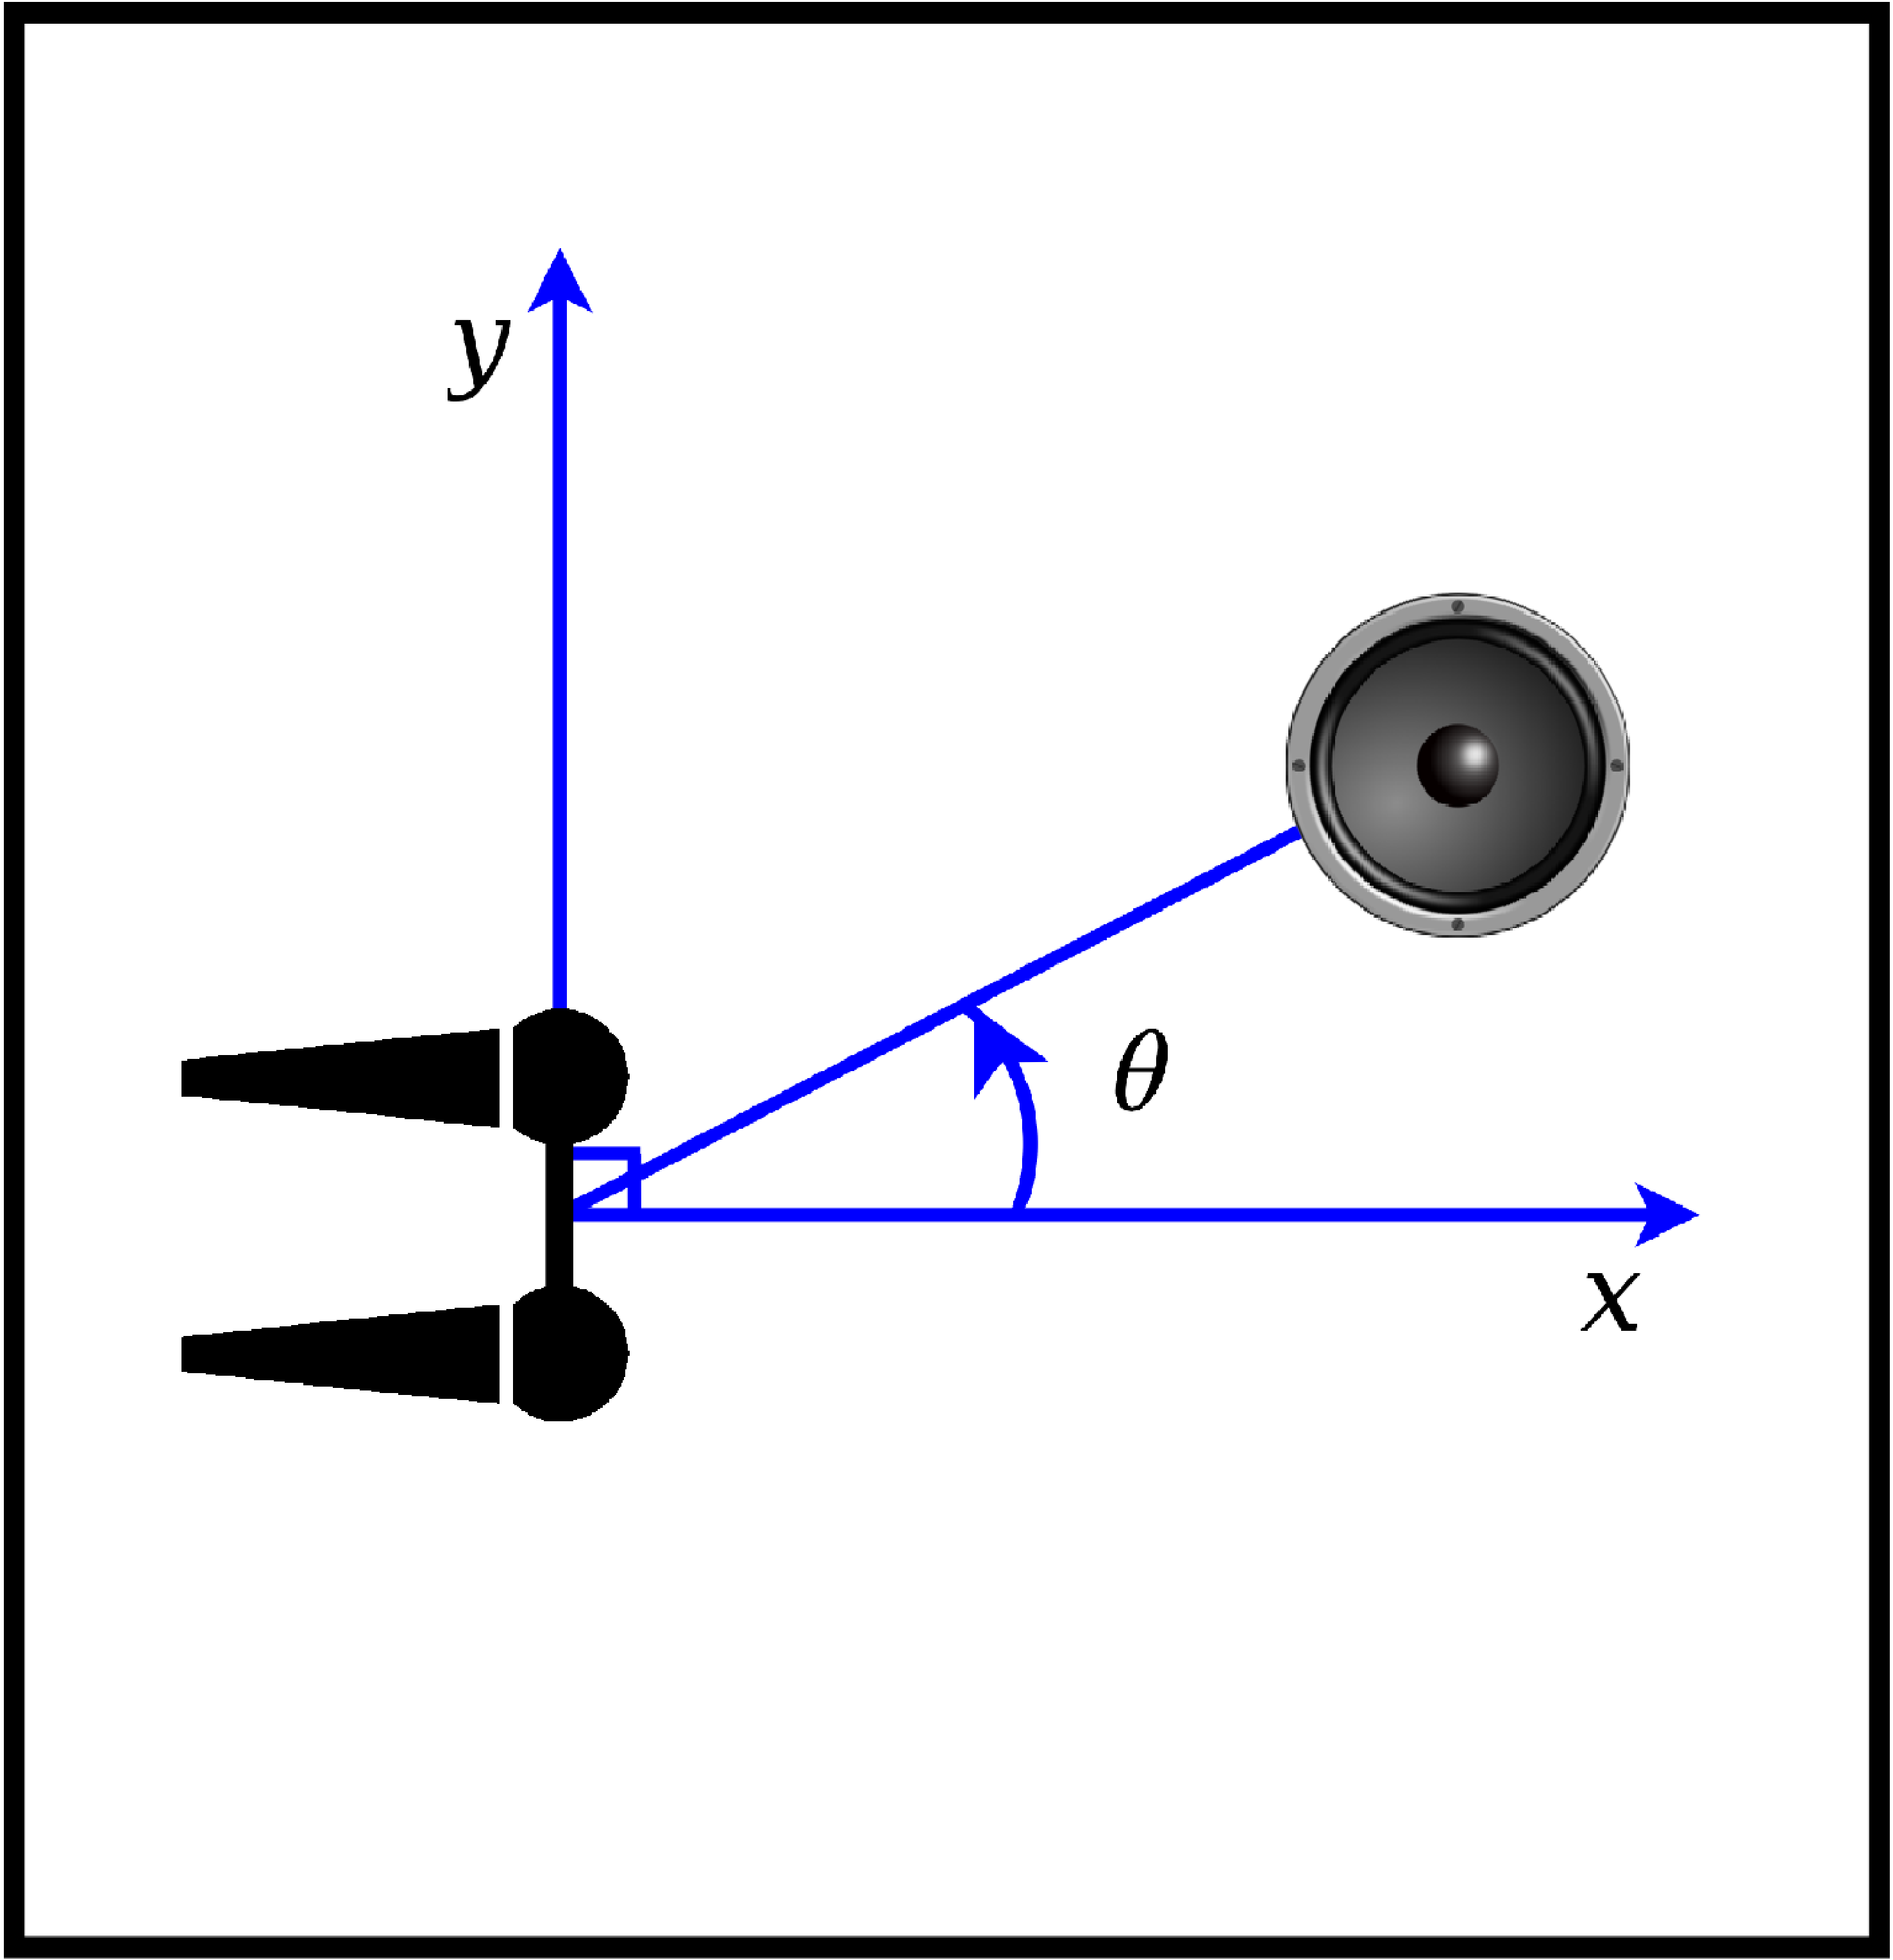
\includegraphics[width=50mm]{recording_room_final}
      \caption { A microphone array with two microphones in an anechoic chamber.
      The polar angle with respect to the $x$-axis is $\theta$. }
          \label{fig:recording_room_final}
  \end{center}
\end{figure}
%
%
Before discussing the Phase-Distortion TRaining (PDTR)/
Spectral-Distortion TRaining (SDTR) model in detail
in the next section, we briefly examine how the magnitude-phase distortion
occurs with real recording. Let us consider
a configuration for recording in an "anechoic" chamber as shown in Fig.
\ref{fig:recording_room_final}. The target sound source is a high-quality
loud speaker in this anechoic chamber without other noisy sound sources.
In this setup, the distance between two microphones was 5.1 $cm$.
The distance from the target sound source to the microphone array is two
meters. Let us denote the polar angle by $\theta$, which is the angle
between the perpendicular bisector to the line connecting two microphones
and the line connecting the center of the array to the loud speaker.
Fig. \ref{fig:microphone_responses} show a two-channel microphone
response obtained in this configuration with $\theta=0^{o}$.
Impulse responses were obtained using the method proposed by A. Farina
\cite{A_Frina_AES_2000}.
%
%
\begin{figure}
  \begin{center}
    \subfigure[\label{fig:time_domain_response_2_91_90_rir_anechoic_16k}] {
    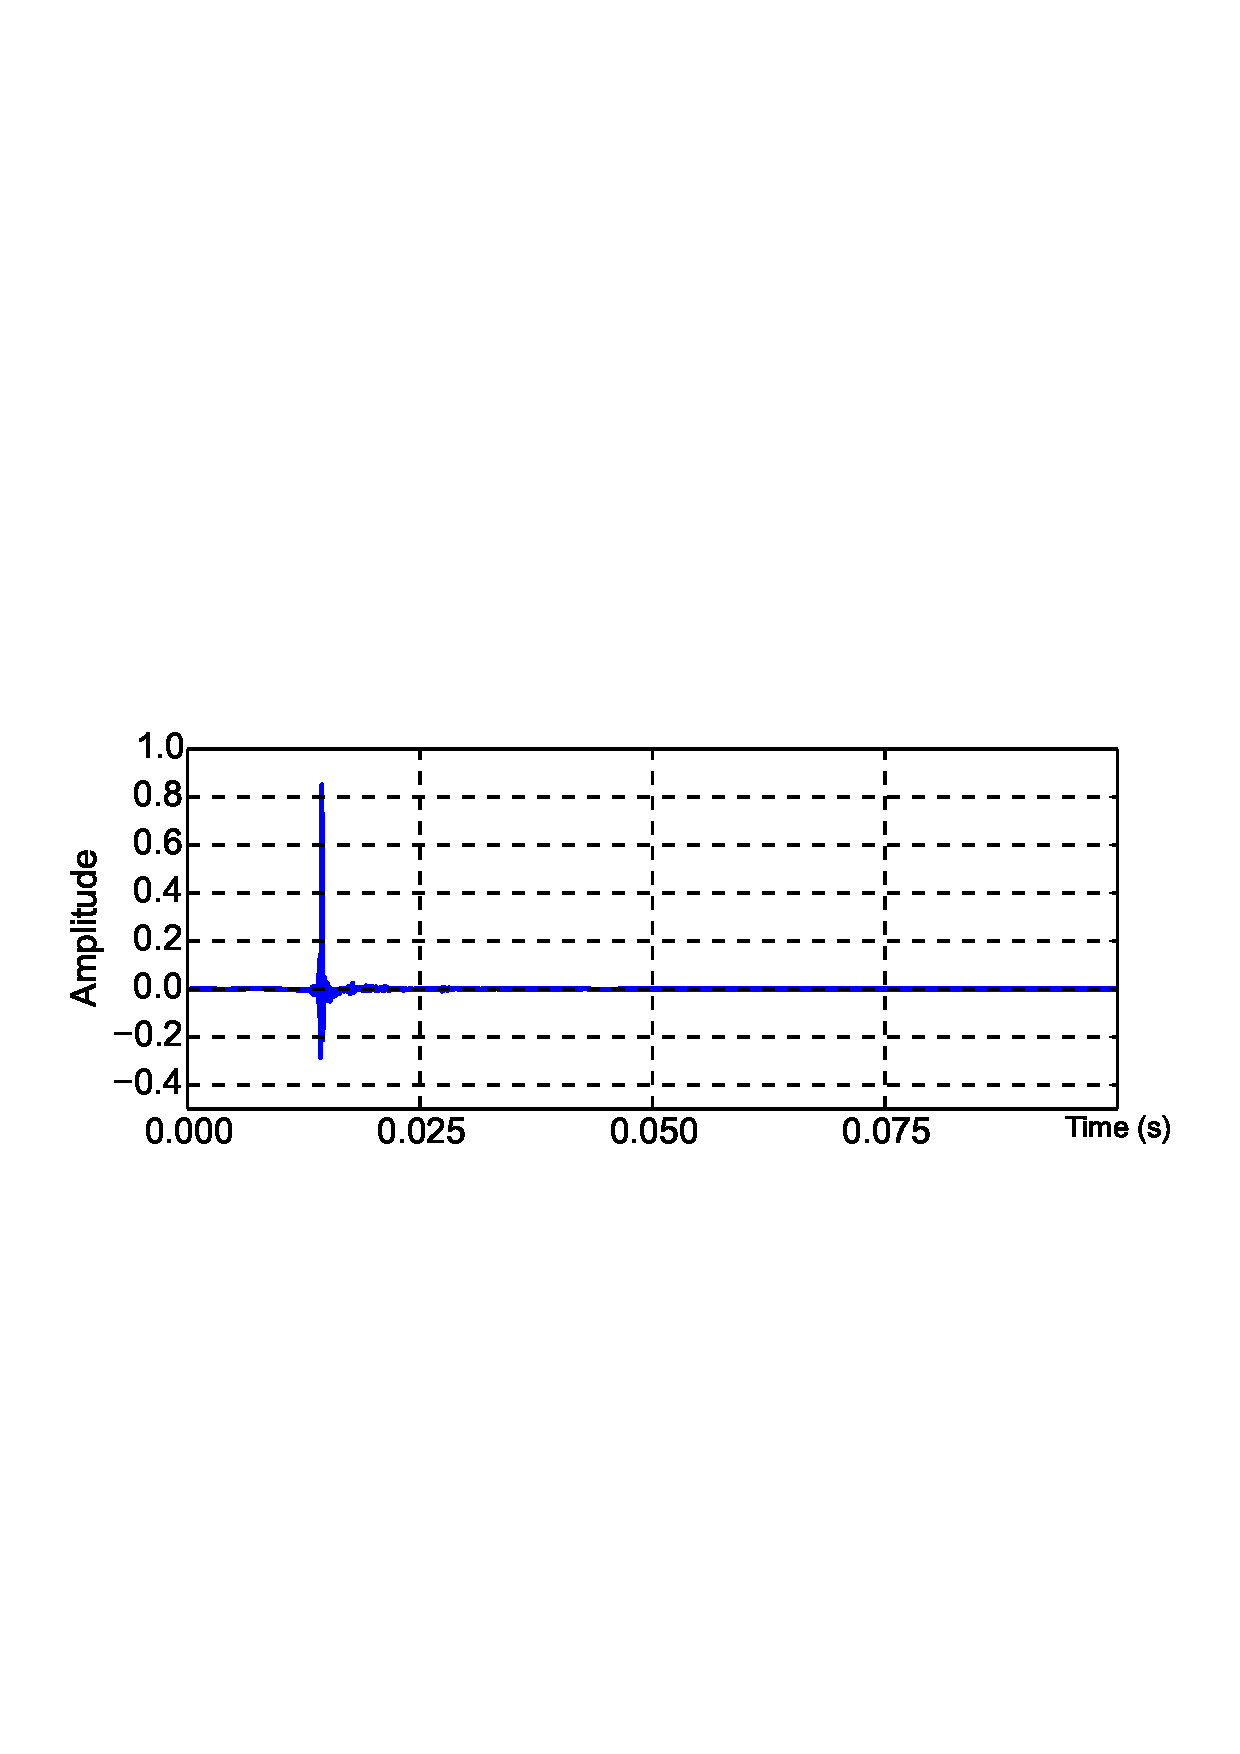
\includegraphics[width=70mm]{time_domain_response_2_91_90_rir_anechoic_16k}}
  \subfigure[\label{fig:magnitude_response_2_91_90_rir_anechoic_16k}] {
    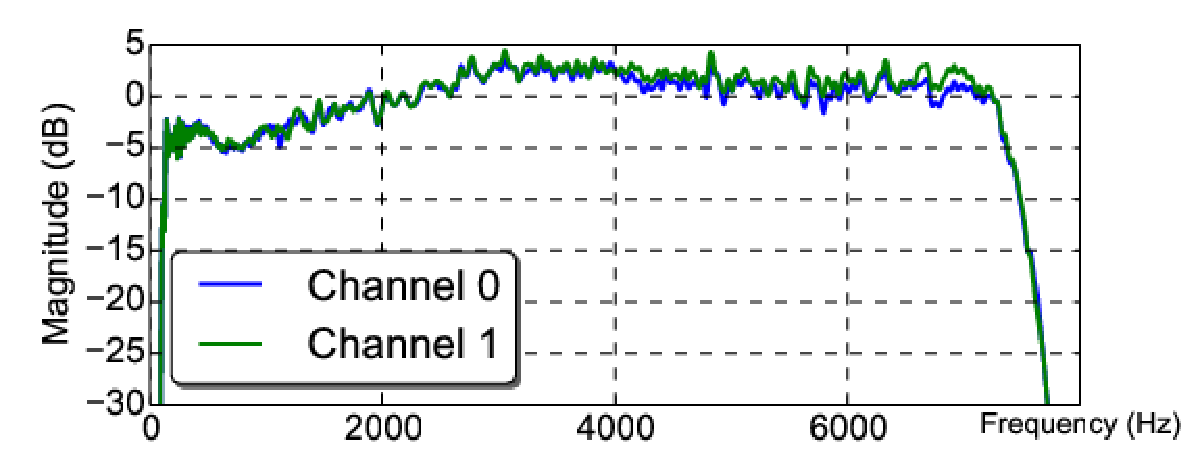
\includegraphics[width=70mm]{magnitude_response_2_91_90_rir_anechoic_16k}}
  \subfigure[\label{fig:phase_response_2_91_90_rir_anechoic_16k}] {
    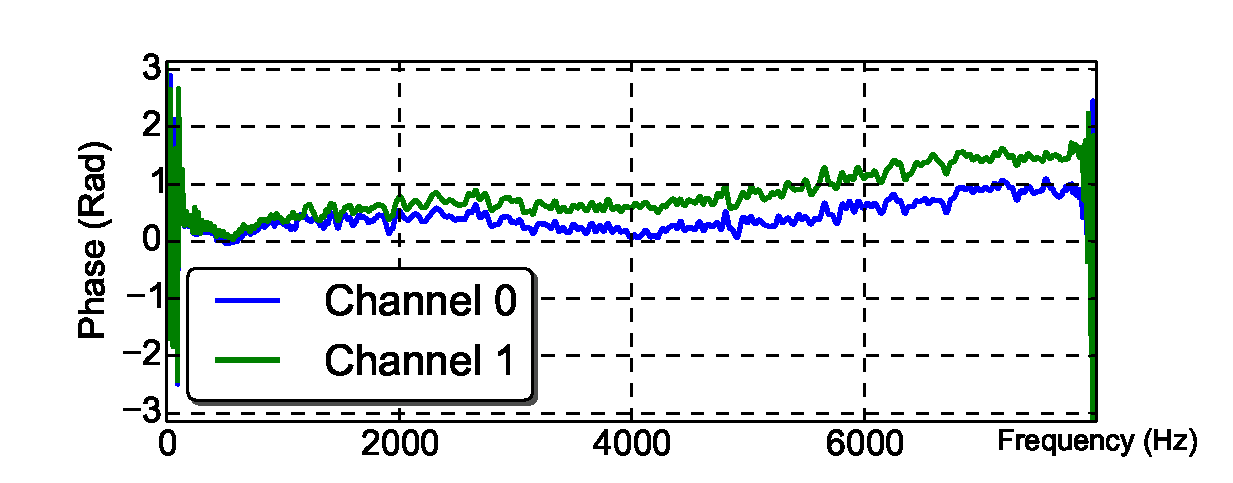
\includegraphics[width=70mm]{phase_response_2_91_90_rir_anechoic_16k}}
  \caption {\label{fig:microphone_responses} \emph{ 
    (a) A microphone response recorded in an anechoic chamber.
    (b) Magnitudes of two microphone transfer functions from a single microphone array,
    and (c) Phases of two microphone transfer functions from a single microphone array.}}
  \end{center}
\end{figure}
%
%
%
As shown in Fig. \ref{fig:magnitude_response_2_91_90_rir_anechoic_16k}
and Fig. \ref{fig:target_to_mic_distribution}, the magnitude and the phase
responses are different from the ideal responses, which is the all-pass
zero-phase response. Since the polar angle $\theta=0^{0}$ in this case,
the phase components from two microphones are the same in the ideal case.
However, as shown in Fig. \ref{fig:phase_response_2_91_90_rir_anechoic_16k},
the phases from two microphones are not the same.
%
The relationship between the phase difference and Angle of Arrival (AoA) $\theta$
at discrete frequency $k$ is given by the following equation
\cite{C_Kim_INTERSPEECH_2015, C_Kim_ICASSP_2012_2}:
\begin{align}
  \theta(\omega_k) = \arcsin \left( \frac{\Delta \phi (\omega_k) c_0}{\omega_k d_m f_s}  \right)
\end{align}
where $\omega_k$ is the discrete frequency, $\Delta \phi (\omega_k)$ is the
phase difference at this frequency $\omega_k$. $f_s$, $d_m$ and $c_0$ are
sampling rates in Hz, the distance between two microphones, and
the speed of sound, respectively. Using this equation, the estimated
Angle of Arrivals(AoAs) are obtained in Fig. \ref{fig:estimated_aoa}
for three different locations with
the true polar angle $\theta$ of $45^{o}$, $0^{0}$, and $-45^{o}$ respectively.
From this figure, the phase distortion of real hardware may be easily observed.

\begin{figure}
  \begin{center}
  \subfigure[\label{fig:room_snr_db_distribution}] {
    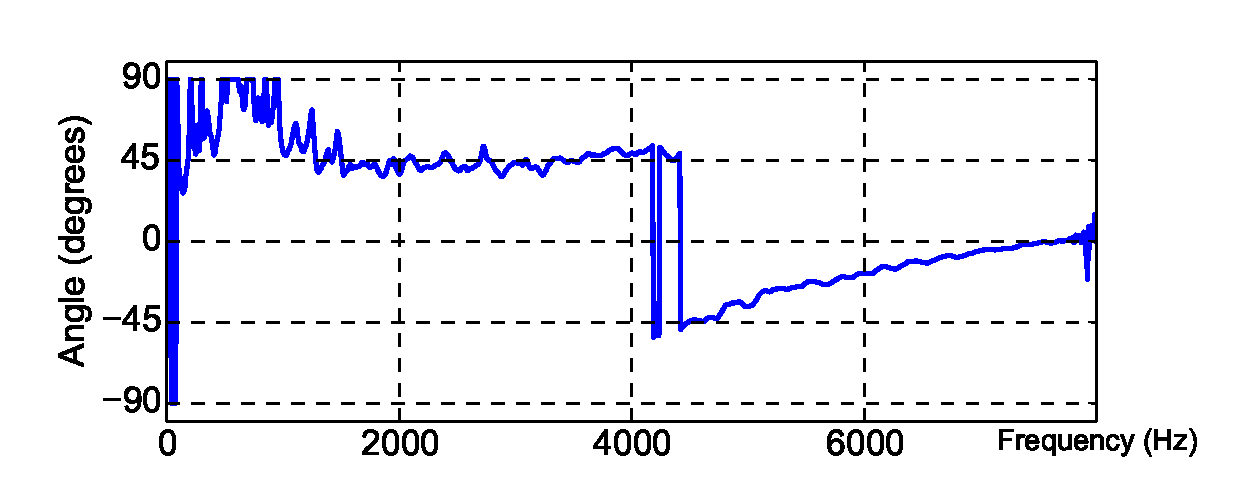
\includegraphics[width=70mm]{estimated_angle_2_45_90_rir_anechoic_16k}
  %  \caption{$\theta=45^{o}$}
  }
  \subfigure[\label{fig:estimated_angle_2_91_90_rir_anechoic_16k}] {
    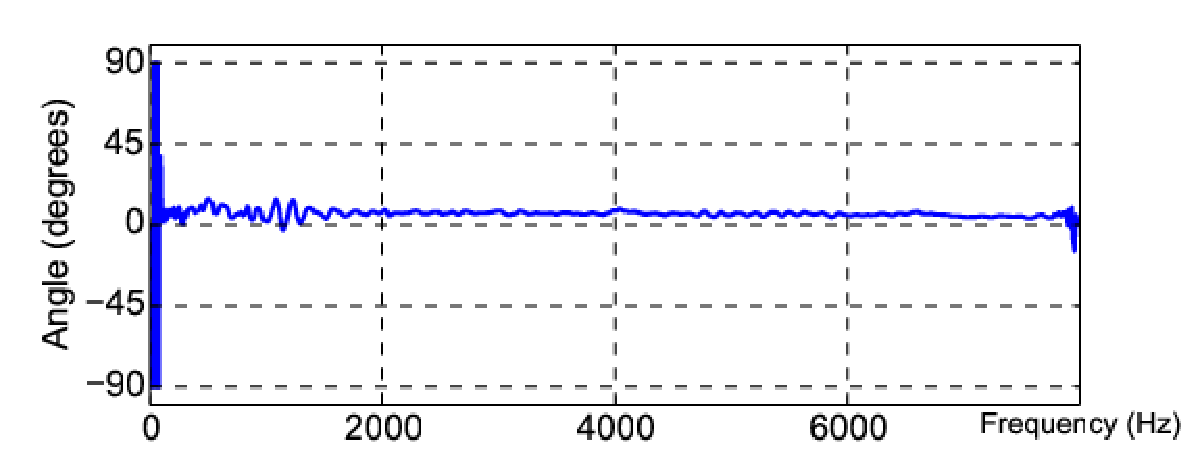
\includegraphics[width=70mm]{estimated_angle_2_91_90_rir_anechoic_16k}}
  \subfigure[\label{fig:target_to_mic_distribution}] {
    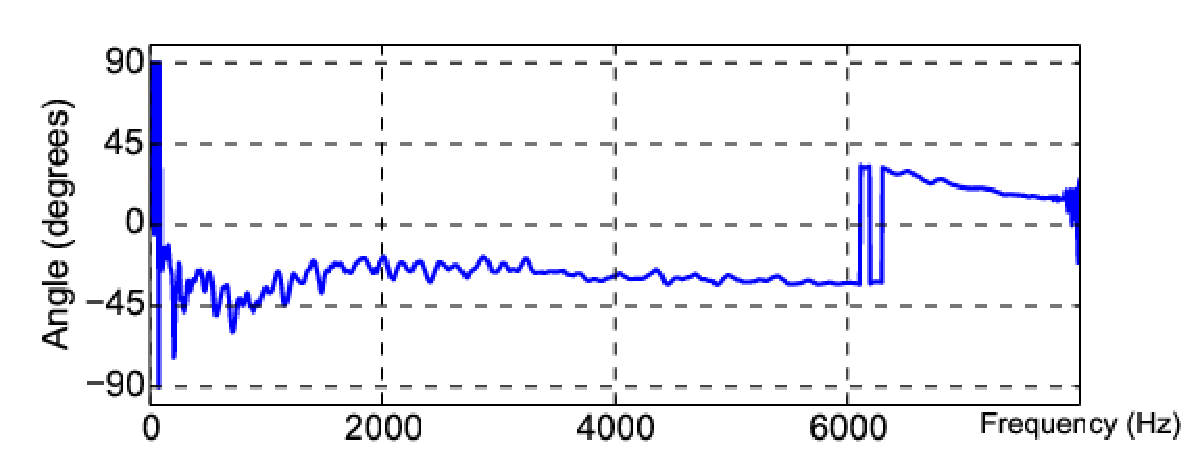
\includegraphics[width=70mm]{estimated_angle_2_135_90_rir_anechoic_16k}}
  \caption {\label{fig:estimated_aoa}\emph{ The estimated Angle of Arrival when the true polar
    angle $\theta$ is (a) $45^{o}$ (b) $0^{o}$, and (c) $-45^{o}$. }}
  \end{center}
\end{figure}
%
%
%
\section{Spectral-Distortion TRaining (SDTR)/Phase-Distortion TRaining (PDTR)}

In this section, we explain the entire structure of
Spectral-Distortion TRaining (SDTR)/Phase-Distortion TRaining (PDTR).
PDTR is a subset of SDTR where distortion is only
applied to the phase component without modifying the magnitude component
of complex features.
PDTR is devised for enhancing the robustness of phase-sensitive
multi-microphone neural network models such as
\cite{ B_Li_INTERSPEECH_2017_1, T_Sainath_INTERSPEECH_2015_1}.
Fig. \ref{fig:entire_diagram} shows the structure of the acoustic model
pipeline used in the experiment in Sec. \label{sec:experimental_results}.
This pipeline is based on the architecture described in
\cite{T_Sainath_ICASSP_2016_1, B_Li_INTERSPEECH_2017_1}. To make
the phase-sensitive multi-channel feature more robust, we add
the Spectral Distortion Model (SDM) to each channel. The actual equation
we use for this SDM is described in \eqref{eq:spectrum_distortion}.
The first stage of the pipeline in Fig \ref{fig:entire_diagram} is
is the room simulator to  generate millions of different utterances
in millions different virtual rooms \cite{C_Kim_INTERSPEECH_2017_1}.
In the room simulation system, we assume that all microphones
have the same zero-phase all-pass response.
This assumption is not true for real microphone arrays as observed in Sec.
\ref{sec:spectral_distortion}
%
\begin{figure}[t]
  \begin{center}
    \resizebox{50mm}{!}{% Graphic for TeX using PGF
% Title: /google/src/cloud/chanwcom/chanwcom-speech9999/google3/experimental/users/chanwcom/my_papers/papers_working/icml_2018_feature_mapping_spl/figures/entire_diagram.dia
% Creator: Dia v0.97.2
% CreationDate: Fri Nov 24 23:29:46 2017
% For: chanwcom
% \usepackage{tikz}
% The following commands are not supported in PSTricks at present
% We define them conditionally, so when they are implemented,
% this pgf file will use them.
\ifx\du\undefined
  \newlength{\du}
\fi
\setlength{\du}{15\unitlength}
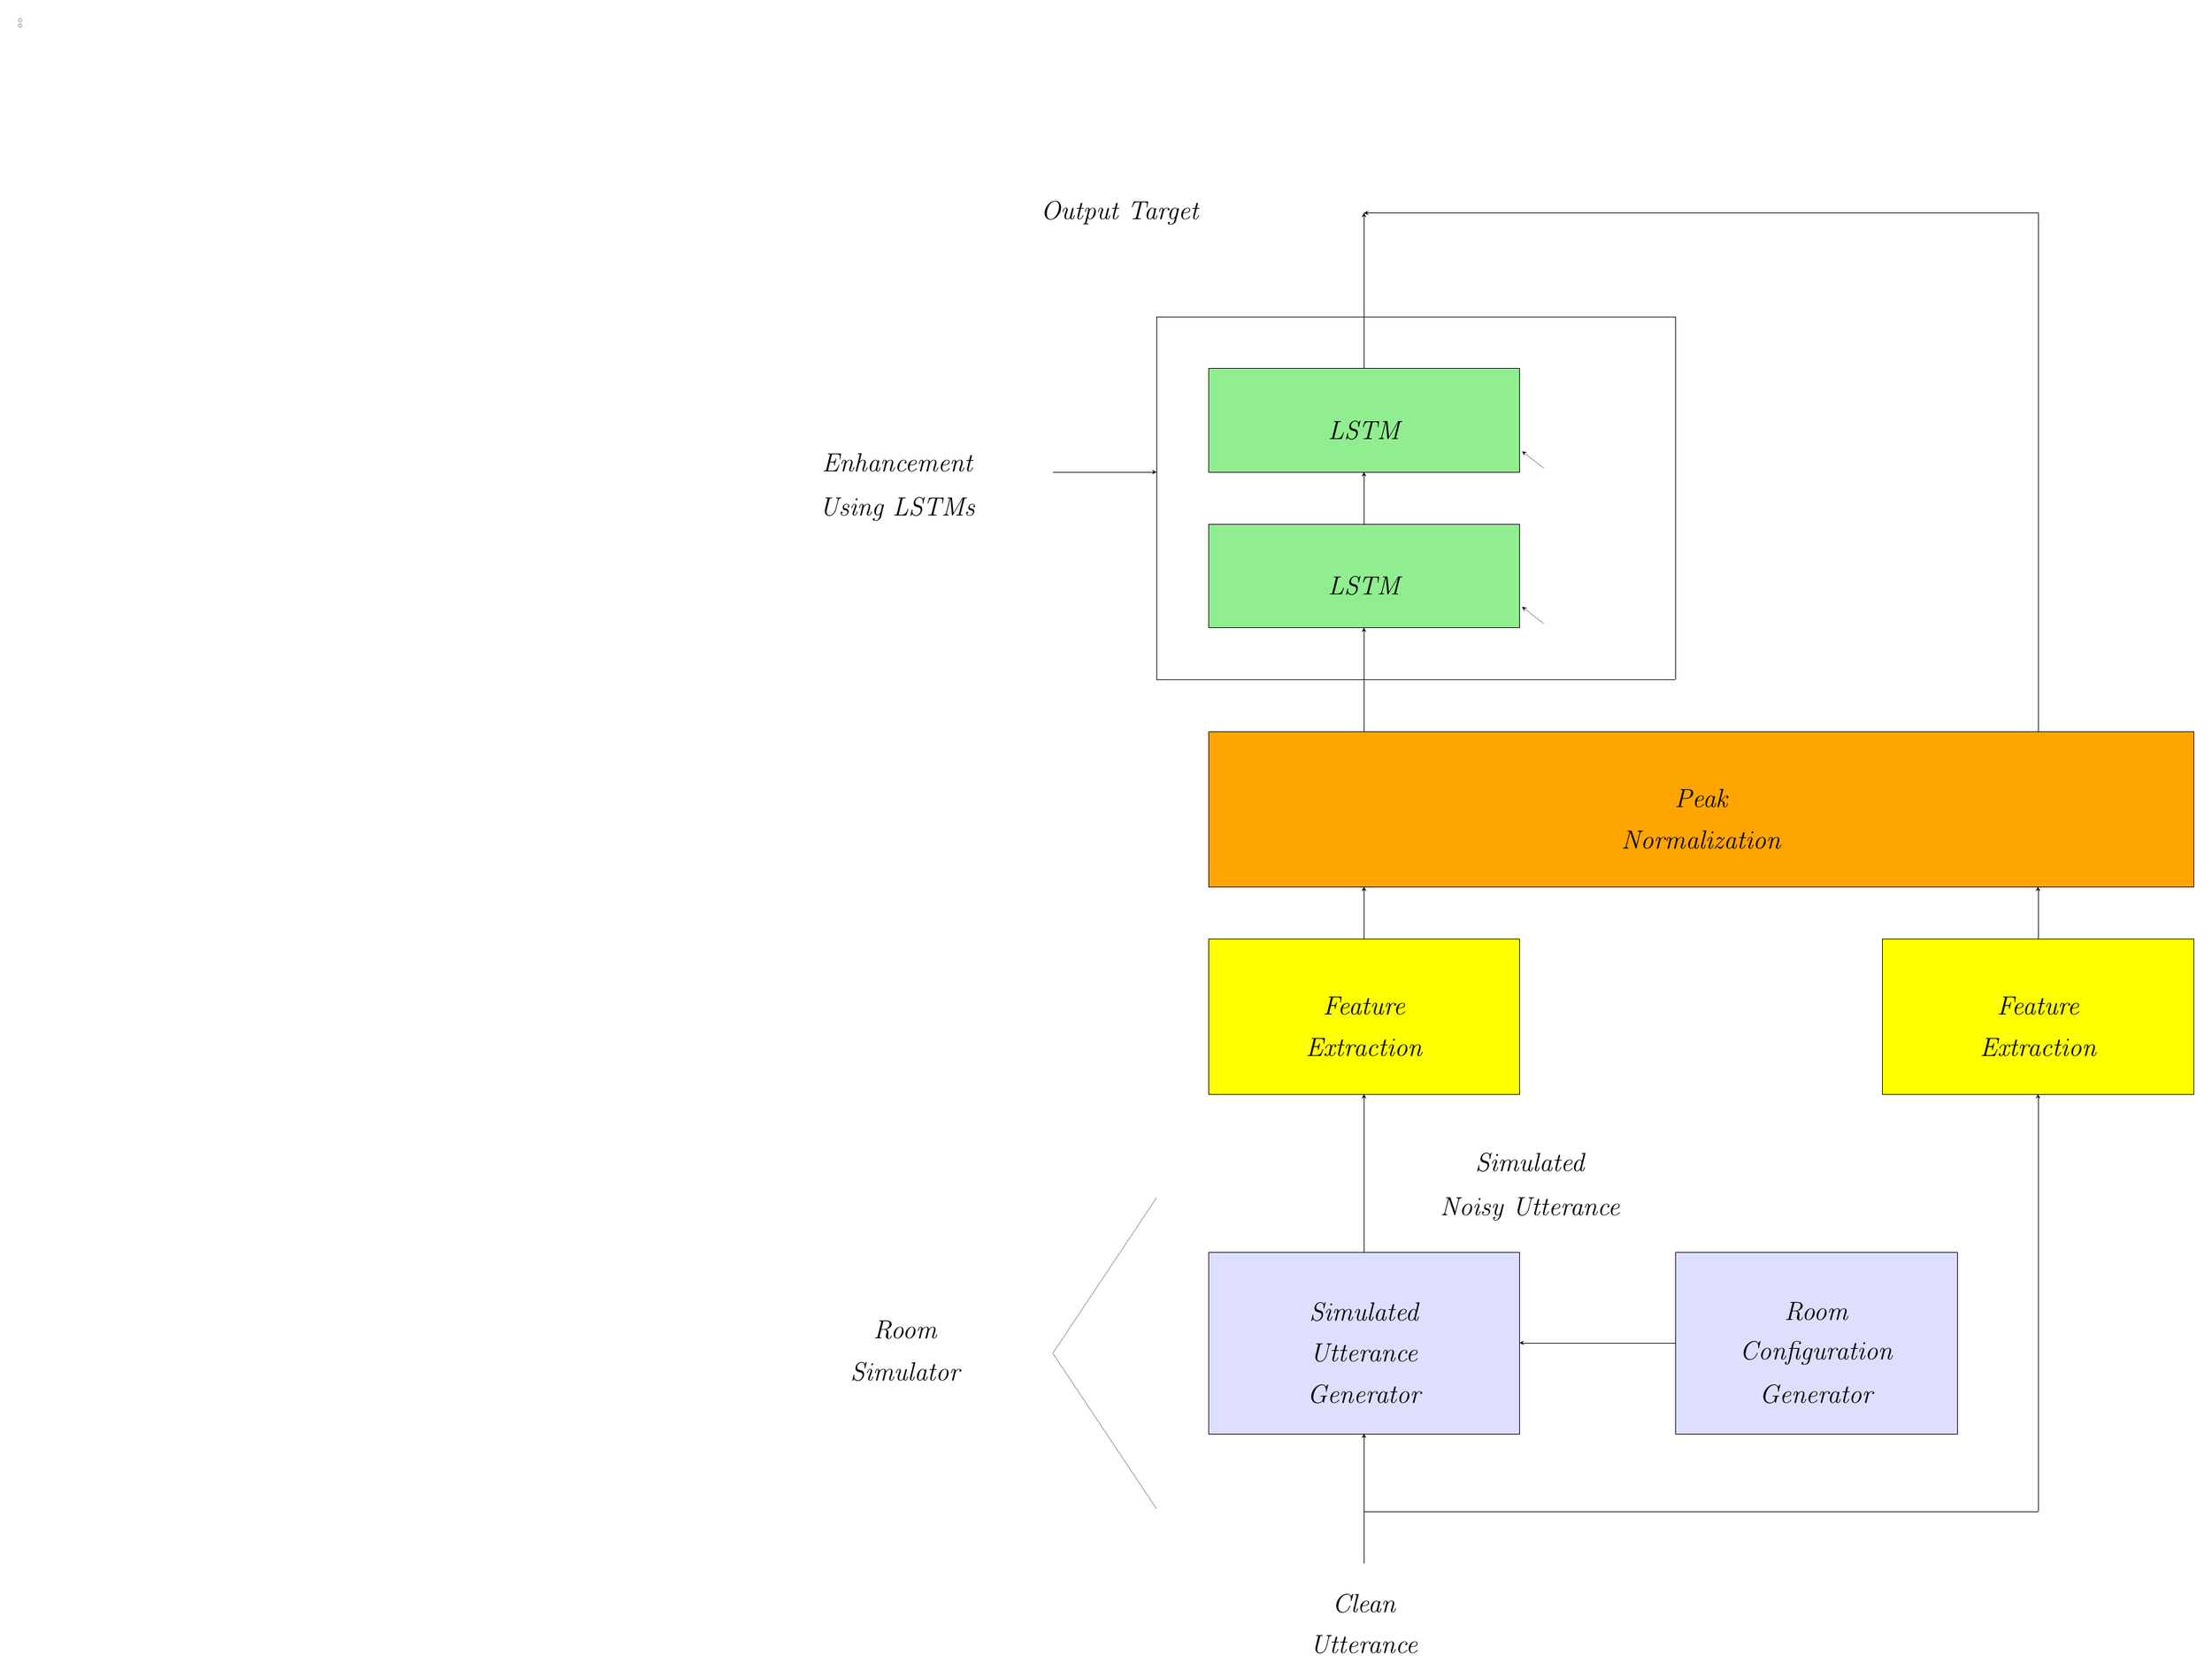
\begin{tikzpicture}
  \tikzstyle{every node}=[font=\Large\itshape]
\pgftransformxscale{1.000000}
\pgftransformyscale{-1.000000}
\definecolor{dialinecolor}{rgb}{0.000000, 0.000000, 0.000000}
\pgfsetstrokecolor{dialinecolor}
\definecolor{dialinecolor}{rgb}{1.000000, 1.000000, 1.000000}
\pgfsetfillcolor{dialinecolor}
\definecolor{dialinecolor}{rgb}{1.000000, 1.000000, 1.000000}
\pgfsetfillcolor{dialinecolor}
\fill (23.000000\du,6.000000\du)--(23.000000\du,13.000000\du)--(33.000000\du,13.000000\du)--(33.000000\du,6.000000\du)--cycle;
\pgfsetlinewidth{0.100000\du}
\pgfsetdash{{\pgflinewidth}{0.200000\du}}{0cm}
\pgfsetdash{{\pgflinewidth}{0.200000\du}}{0cm}
\pgfsetmiterjoin
\definecolor{dialinecolor}{rgb}{0.000000, 0.000000, 0.000000}
\pgfsetstrokecolor{dialinecolor}
\draw (23.000000\du,6.000000\du)--(23.000000\du,13.000000\du)--(33.000000\du,13.000000\du)--(33.000000\du,6.000000\du)--cycle;
% setfont left to latex
\definecolor{dialinecolor}{rgb}{0.000000, 0.000000, 0.000000}
\pgfsetstrokecolor{dialinecolor}
\node at (28.000000\du,9.695000\du){};
\definecolor{dialinecolor}{rgb}{0.870588, 0.870588, 1.000000}
\pgfsetfillcolor{dialinecolor}
\fill (24.000000\du,24.050000\du)--(24.000000\du,27.550000\du)--(30.000000\du,27.550000\du)--(30.000000\du,24.050000\du)--cycle;
\pgfsetlinewidth{0.100000\du}
\pgfsetdash{}{0pt}
\pgfsetdash{}{0pt}
\pgfsetmiterjoin
\definecolor{dialinecolor}{rgb}{0.000000, 0.000000, 0.000000}
\pgfsetstrokecolor{dialinecolor}
\draw (24.000000\du,24.050000\du)--(24.000000\du,27.550000\du)--(30.000000\du,27.550000\du)--(30.000000\du,24.050000\du)--cycle;
% setfont left to latex
\definecolor{dialinecolor}{rgb}{0.000000, 0.000000, 0.000000}
\pgfsetstrokecolor{dialinecolor}
\node at (27.000000\du,25.195000\du){Simulated};
% setfont left to latex
\definecolor{dialinecolor}{rgb}{0.000000, 0.000000, 0.000000}
\pgfsetstrokecolor{dialinecolor}
\node at (27.000000\du,25.995000\du){Utterance};
% setfont left to latex
\definecolor{dialinecolor}{rgb}{0.000000, 0.000000, 0.000000}
\pgfsetstrokecolor{dialinecolor}
\node at (27.000000\du,26.795000\du){Generator};
% setfont left to latex
\definecolor{dialinecolor}{rgb}{0.000000, 0.000000, 0.000000}
\pgfsetstrokecolor{dialinecolor}
\node[anchor=west] at (27.000000\du,25.800000\du){};
\pgfsetlinewidth{0.100000\du}
\pgfsetdash{}{0pt}
\pgfsetdash{}{0pt}
\pgfsetbuttcap
{
\definecolor{dialinecolor}{rgb}{0.000000, 0.000000, 0.000000}
\pgfsetfillcolor{dialinecolor}
% was here!!!
\pgfsetarrowsend{stealth}
\definecolor{dialinecolor}{rgb}{0.000000, 0.000000, 0.000000}
\pgfsetstrokecolor{dialinecolor}
\draw (40.000000\du,29.050000\du)--(40.000000\du,21.000000\du);
}
\pgfsetlinewidth{0.100000\du}
\pgfsetdash{}{0pt}
\pgfsetdash{}{0pt}
\pgfsetbuttcap
{
\definecolor{dialinecolor}{rgb}{0.000000, 0.000000, 0.000000}
\pgfsetfillcolor{dialinecolor}
% was here!!!
\pgfsetarrowsend{stealth}
\definecolor{dialinecolor}{rgb}{0.000000, 0.000000, 0.000000}
\pgfsetstrokecolor{dialinecolor}
\draw (27.000000\du,24.050000\du)--(27.000000\du,21.000000\du);
}
\definecolor{dialinecolor}{rgb}{1.000000, 1.000000, 1.000000}
\pgfsetfillcolor{dialinecolor}
\pgfpathellipse{\pgfpoint{30.850000\du}{11.000000\du}}{\pgfpoint{1.000000\du}{0\du}}{\pgfpoint{0\du}{1.000000\du}}
\pgfusepath{fill}
\pgfsetlinewidth{0.100000\du}
\pgfsetdash{}{0pt}
\pgfsetdash{}{0pt}
\pgfsetmiterjoin
\definecolor{dialinecolor}{rgb}{0.000000, 0.000000, 0.000000}
\pgfsetstrokecolor{dialinecolor}
\pgfpathellipse{\pgfpoint{30.850000\du}{11.000000\du}}{\pgfpoint{1.000000\du}{0\du}}{\pgfpoint{0\du}{1.000000\du}}
\pgfusepath{stroke}
% setfont left to latex
\definecolor{dialinecolor}{rgb}{0.000000, 0.000000, 0.000000}
\pgfsetstrokecolor{dialinecolor}
\node at (30.850000\du,11.195000\du){};
\pgfsetlinewidth{0.100000\du}
\pgfsetdash{}{0pt}
\pgfsetdash{}{0pt}
\pgfsetbuttcap
{
\definecolor{dialinecolor}{rgb}{0.000000, 0.000000, 0.000000}
\pgfsetfillcolor{dialinecolor}
% was here!!!
\pgfsetarrowsend{stealth}
\definecolor{dialinecolor}{rgb}{0.000000, 0.000000, 0.000000}
\pgfsetstrokecolor{dialinecolor}
\draw (30.467300\du,11.923900\du)--(30.050000\du,11.600000\du);
}
\definecolor{dialinecolor}{rgb}{1.000000, 1.000000, 1.000000}
\pgfsetfillcolor{dialinecolor}
\pgfpathellipse{\pgfpoint{30.850000\du}{8.000000\du}}{\pgfpoint{1.000000\du}{0\du}}{\pgfpoint{0\du}{1.000000\du}}
\pgfusepath{fill}
\pgfsetlinewidth{0.100000\du}
\pgfsetdash{}{0pt}
\pgfsetdash{}{0pt}
\pgfsetmiterjoin
\definecolor{dialinecolor}{rgb}{0.000000, 0.000000, 0.000000}
\pgfsetstrokecolor{dialinecolor}
\pgfpathellipse{\pgfpoint{30.850000\du}{8.000000\du}}{\pgfpoint{1.000000\du}{0\du}}{\pgfpoint{0\du}{1.000000\du}}
\pgfusepath{stroke}
% setfont left to latex
\definecolor{dialinecolor}{rgb}{0.000000, 0.000000, 0.000000}
\pgfsetstrokecolor{dialinecolor}
\node at (30.850000\du,8.195000\du){};
\pgfsetlinewidth{0.100000\du}
\pgfsetdash{}{0pt}
\pgfsetdash{}{0pt}
\pgfsetbuttcap
{
\definecolor{dialinecolor}{rgb}{0.000000, 0.000000, 0.000000}
\pgfsetfillcolor{dialinecolor}
% was here!!!
\pgfsetarrowsend{stealth}
\definecolor{dialinecolor}{rgb}{0.000000, 0.000000, 0.000000}
\pgfsetstrokecolor{dialinecolor}
\draw (30.467300\du,8.923880\du)--(30.050000\du,8.600000\du);
}
\definecolor{dialinecolor}{rgb}{0.564706, 0.933333, 0.564706}
\pgfsetfillcolor{dialinecolor}
\fill (24.000000\du,7.000000\du)--(24.000000\du,9.000000\du)--(30.000000\du,9.000000\du)--(30.000000\du,7.000000\du)--cycle;
\pgfsetlinewidth{0.100000\du}
\pgfsetdash{}{0pt}
\pgfsetdash{}{0pt}
\pgfsetmiterjoin
\definecolor{dialinecolor}{rgb}{0.000000, 0.000000, 0.000000}
\pgfsetstrokecolor{dialinecolor}
\draw (24.000000\du,7.000000\du)--(24.000000\du,9.000000\du)--(30.000000\du,9.000000\du)--(30.000000\du,7.000000\du)--cycle;
% setfont left to latex
\definecolor{dialinecolor}{rgb}{0.000000, 0.000000, 0.000000}
\pgfsetstrokecolor{dialinecolor}
\node at (27.000000\du,8.195000\du){LSTM};
\definecolor{dialinecolor}{rgb}{0.564706, 0.933333, 0.564706}
\pgfsetfillcolor{dialinecolor}
\fill (24.000000\du,10.000000\du)--(24.000000\du,12.000000\du)--(30.000000\du,12.000000\du)--(30.000000\du,10.000000\du)--cycle;
\pgfsetlinewidth{0.100000\du}
\pgfsetdash{}{0pt}
\pgfsetdash{}{0pt}
\pgfsetmiterjoin
\definecolor{dialinecolor}{rgb}{0.000000, 0.000000, 0.000000}
\pgfsetstrokecolor{dialinecolor}
\draw (24.000000\du,10.000000\du)--(24.000000\du,12.000000\du)--(30.000000\du,12.000000\du)--(30.000000\du,10.000000\du)--cycle;
% setfont left to latex
\definecolor{dialinecolor}{rgb}{0.000000, 0.000000, 0.000000}
\pgfsetstrokecolor{dialinecolor}
\node at (27.000000\du,11.195000\du){LSTM};
\pgfsetlinewidth{0.100000\du}
\pgfsetdash{}{0pt}
\pgfsetdash{}{0pt}
\pgfsetbuttcap
{
\definecolor{dialinecolor}{rgb}{0.000000, 0.000000, 0.000000}
\pgfsetfillcolor{dialinecolor}
% was here!!!
\pgfsetarrowsend{stealth}
\definecolor{dialinecolor}{rgb}{0.000000, 0.000000, 0.000000}
\pgfsetstrokecolor{dialinecolor}
\draw (27.000000\du,14.000000\du)--(27.000000\du,12.000000\du);
}
\pgfsetlinewidth{0.100000\du}
\pgfsetdash{}{0pt}
\pgfsetdash{}{0pt}
\pgfsetbuttcap
{
\definecolor{dialinecolor}{rgb}{0.000000, 0.000000, 0.000000}
\pgfsetfillcolor{dialinecolor}
% was here!!!
\pgfsetarrowsend{stealth}
\definecolor{dialinecolor}{rgb}{0.000000, 0.000000, 0.000000}
\pgfsetstrokecolor{dialinecolor}
\draw (27.000000\du,10.000000\du)--(27.000000\du,9.000000\du);
}
\pgfsetlinewidth{0.100000\du}
\pgfsetdash{}{0pt}
\pgfsetdash{}{0pt}
\pgfsetbuttcap
{
\definecolor{dialinecolor}{rgb}{0.000000, 0.000000, 0.000000}
\pgfsetfillcolor{dialinecolor}
% was here!!!
\definecolor{dialinecolor}{rgb}{0.000000, 0.000000, 0.000000}
\pgfsetstrokecolor{dialinecolor}
\draw (40.000000\du,14.000000\du)--(40.000000\du,4.000000\du);
}
% setfont left to latex
\definecolor{dialinecolor}{rgb}{0.000000, 0.000000, 0.000000}
\pgfsetstrokecolor{dialinecolor}
\node[anchor=west] at (20.650000\du,4.000000\du){Output Target};
\definecolor{dialinecolor}{rgb}{0.870588, 0.870588, 1.000000}
\pgfsetfillcolor{dialinecolor}
\fill (33.000000\du,24.050000\du)--(33.000000\du,27.550000\du)--(38.440000\du,27.550000\du)--(38.440000\du,24.050000\du)--cycle;
\pgfsetlinewidth{0.100000\du}
\pgfsetdash{}{0pt}
\pgfsetdash{}{0pt}
\pgfsetmiterjoin
\definecolor{dialinecolor}{rgb}{0.000000, 0.000000, 0.000000}
\pgfsetstrokecolor{dialinecolor}
\draw (33.000000\du,24.050000\du)--(33.000000\du,27.550000\du)--(38.440000\du,27.550000\du)--(38.440000\du,24.050000\du)--cycle;
% setfont left to latex
\definecolor{dialinecolor}{rgb}{0.000000, 0.000000, 0.000000}
\pgfsetstrokecolor{dialinecolor}
\node at (35.720000\du,25.195000\du){Room};
% setfont left to latex
\definecolor{dialinecolor}{rgb}{0.000000, 0.000000, 0.000000}
\pgfsetstrokecolor{dialinecolor}
\node at (35.720000\du,25.995000\du){Configuration};
% setfont left to latex
\definecolor{dialinecolor}{rgb}{0.000000, 0.000000, 0.000000}
\pgfsetstrokecolor{dialinecolor}
\node at (35.720000\du,26.795000\du){Generator};
\pgfsetlinewidth{0.100000\du}
\pgfsetdash{}{0pt}
\pgfsetdash{}{0pt}
\pgfsetbuttcap
{
\definecolor{dialinecolor}{rgb}{0.000000, 0.000000, 0.000000}
\pgfsetfillcolor{dialinecolor}
% was here!!!
\pgfsetarrowsend{stealth}
\definecolor{dialinecolor}{rgb}{0.000000, 0.000000, 0.000000}
\pgfsetstrokecolor{dialinecolor}
\draw (33.000000\du,25.800000\du)--(30.000000\du,25.800000\du);
}
\definecolor{dialinecolor}{rgb}{1.000000, 1.000000, 0.000000}
\pgfsetfillcolor{dialinecolor}
\fill (37.000000\du,18.000000\du)--(37.000000\du,21.000000\du)--(43.000000\du,21.000000\du)--(43.000000\du,18.000000\du)--cycle;
\pgfsetlinewidth{0.100000\du}
\pgfsetdash{}{0pt}
\pgfsetdash{}{0pt}
\pgfsetmiterjoin
\definecolor{dialinecolor}{rgb}{0.000000, 0.000000, 0.000000}
\pgfsetstrokecolor{dialinecolor}
\draw (37.000000\du,18.000000\du)--(37.000000\du,21.000000\du)--(43.000000\du,21.000000\du)--(43.000000\du,18.000000\du)--cycle;
% setfont left to latex
\definecolor{dialinecolor}{rgb}{0.000000, 0.000000, 0.000000}
\pgfsetstrokecolor{dialinecolor}
\node at (40.000000\du,19.295000\du){Feature};
% setfont left to latex
\definecolor{dialinecolor}{rgb}{0.000000, 0.000000, 0.000000}
\pgfsetstrokecolor{dialinecolor}
\node at (40.000000\du,20.095000\du){Extraction};
\pgfsetlinewidth{0.100000\du}
\pgfsetdash{}{0pt}
\pgfsetdash{}{0pt}
\pgfsetbuttcap
{
\definecolor{dialinecolor}{rgb}{0.000000, 0.000000, 0.000000}
\pgfsetfillcolor{dialinecolor}
% was here!!!
\definecolor{dialinecolor}{rgb}{0.000000, 0.000000, 0.000000}
\pgfsetstrokecolor{dialinecolor}
\draw (27.000000\du,29.050000\du)--(40.000000\du,29.050000\du);
}
\definecolor{dialinecolor}{rgb}{1.000000, 1.000000, 0.000000}
\pgfsetfillcolor{dialinecolor}
\fill (24.000000\du,18.000000\du)--(24.000000\du,21.000000\du)--(30.000000\du,21.000000\du)--(30.000000\du,18.000000\du)--cycle;
\pgfsetlinewidth{0.100000\du}
\pgfsetdash{}{0pt}
\pgfsetdash{}{0pt}
\pgfsetmiterjoin
\definecolor{dialinecolor}{rgb}{0.000000, 0.000000, 0.000000}
\pgfsetstrokecolor{dialinecolor}
\draw (24.000000\du,18.000000\du)--(24.000000\du,21.000000\du)--(30.000000\du,21.000000\du)--(30.000000\du,18.000000\du)--cycle;
% setfont left to latex
\definecolor{dialinecolor}{rgb}{0.000000, 0.000000, 0.000000}
\pgfsetstrokecolor{dialinecolor}
\node at (27.000000\du,19.295000\du){Feature};
% setfont left to latex
\definecolor{dialinecolor}{rgb}{0.000000, 0.000000, 0.000000}
\pgfsetstrokecolor{dialinecolor}
\node at (27.000000\du,20.095000\du){Extraction};
\pgfsetlinewidth{0.100000\du}
\pgfsetdash{}{0pt}
\pgfsetdash{}{0pt}
\pgfsetbuttcap
{
\definecolor{dialinecolor}{rgb}{0.000000, 0.000000, 0.000000}
\pgfsetfillcolor{dialinecolor}
% was here!!!
\pgfsetarrowsend{stealth}
\definecolor{dialinecolor}{rgb}{0.000000, 0.000000, 0.000000}
\pgfsetstrokecolor{dialinecolor}
\draw (40.000000\du,18.000000\du)--(40.000000\du,17.000000\du);
}
\definecolor{dialinecolor}{rgb}{1.000000, 0.647059, 0.000000}
\pgfsetfillcolor{dialinecolor}
\fill (24.000000\du,14.000000\du)--(24.000000\du,17.000000\du)--(43.000000\du,17.000000\du)--(43.000000\du,14.000000\du)--cycle;
\pgfsetlinewidth{0.100000\du}
\pgfsetdash{}{0pt}
\pgfsetdash{}{0pt}
\pgfsetmiterjoin
\definecolor{dialinecolor}{rgb}{0.000000, 0.000000, 0.000000}
\pgfsetstrokecolor{dialinecolor}
\draw (24.000000\du,14.000000\du)--(24.000000\du,17.000000\du)--(43.000000\du,17.000000\du)--(43.000000\du,14.000000\du)--cycle;
% setfont left to latex
\definecolor{dialinecolor}{rgb}{0.000000, 0.000000, 0.000000}
\pgfsetstrokecolor{dialinecolor}
\node at (33.500000\du,15.295000\du){Peak};
% setfont left to latex
\definecolor{dialinecolor}{rgb}{0.000000, 0.000000, 0.000000}
\pgfsetstrokecolor{dialinecolor}
\node at (33.500000\du,16.095000\du){Normalization};
\pgfsetlinewidth{0.100000\du}
\pgfsetdash{}{0pt}
\pgfsetdash{}{0pt}
\pgfsetbuttcap
{
\definecolor{dialinecolor}{rgb}{0.000000, 0.000000, 0.000000}
\pgfsetfillcolor{dialinecolor}
% was here!!!
\pgfsetarrowsend{stealth}
\definecolor{dialinecolor}{rgb}{0.000000, 0.000000, 0.000000}
\pgfsetstrokecolor{dialinecolor}
\draw (27.000000\du,18.000000\du)--(27.000000\du,17.000000\du);
}
\pgfsetlinewidth{0.100000\du}
\pgfsetdash{}{0pt}
\pgfsetdash{}{0pt}
\pgfsetbuttcap
{
\definecolor{dialinecolor}{rgb}{0.000000, 0.000000, 0.000000}
\pgfsetfillcolor{dialinecolor}
% was here!!!
\pgfsetarrowsend{stealth}
\definecolor{dialinecolor}{rgb}{0.000000, 0.000000, 0.000000}
\pgfsetstrokecolor{dialinecolor}
\draw (27.000000\du,30.050000\du)--(27.000000\du,27.550000\du);
}
\pgfsetlinewidth{0.100000\du}
\pgfsetdash{}{0pt}
\pgfsetdash{}{0pt}
\pgfsetbuttcap
{
\definecolor{dialinecolor}{rgb}{0.000000, 0.000000, 0.000000}
\pgfsetfillcolor{dialinecolor}
% was here!!!
\pgfsetarrowsend{stealth}
\definecolor{dialinecolor}{rgb}{0.000000, 0.000000, 0.000000}
\pgfsetstrokecolor{dialinecolor}
\draw (40.000000\du,4.000000\du)--(27.000000\du,4.000000\du);
}
\pgfsetlinewidth{0.100000\du}
\pgfsetdash{}{0pt}
\pgfsetdash{}{0pt}
\pgfsetbuttcap
{
\definecolor{dialinecolor}{rgb}{0.000000, 0.000000, 0.000000}
\pgfsetfillcolor{dialinecolor}
% was here!!!
\pgfsetarrowsend{stealth}
\definecolor{dialinecolor}{rgb}{0.000000, 0.000000, 0.000000}
\pgfsetstrokecolor{dialinecolor}
\draw (27.000000\du,7.000000\du)--(27.000000\du,4.000000\du);
}
\pgfsetlinewidth{0.100000\du}
\pgfsetdash{}{0pt}
\pgfsetdash{}{0pt}
\pgfsetbuttcap
{
\definecolor{dialinecolor}{rgb}{0.000000, 0.000000, 0.000000}
\pgfsetfillcolor{dialinecolor}
% was here!!!
\definecolor{dialinecolor}{rgb}{0.000000, 0.000000, 0.000000}
\pgfsetstrokecolor{dialinecolor}
\draw (23.000000\du,23.000000\du)--(21.000000\du,26.000000\du);
}
\pgfsetlinewidth{0.100000\du}
\pgfsetdash{}{0pt}
\pgfsetdash{}{0pt}
\pgfsetbuttcap
{
\definecolor{dialinecolor}{rgb}{0.000000, 0.000000, 0.000000}
\pgfsetfillcolor{dialinecolor}
% was here!!!
\definecolor{dialinecolor}{rgb}{0.000000, 0.000000, 0.000000}
\pgfsetstrokecolor{dialinecolor}
\draw (23.000000\du,29.000000\du)--(21.000000\du,26.000000\du);
}
% setfont left to latex
\definecolor{dialinecolor}{rgb}{0.000000, 0.000000, 0.000000}
\pgfsetstrokecolor{dialinecolor}
\node at (18.150000\du,25.550000\du){Room};
% setfont left to latex
\definecolor{dialinecolor}{rgb}{0.000000, 0.000000, 0.000000}
\pgfsetstrokecolor{dialinecolor}
\node at (18.150000\du,26.350000\du){Simulator};
\pgfsetlinewidth{0.100000\du}
\pgfsetdash{}{0pt}
\pgfsetdash{}{0pt}
\pgfsetbuttcap
{
\definecolor{dialinecolor}{rgb}{0.000000, 0.000000, 0.000000}
\pgfsetfillcolor{dialinecolor}
% was here!!!
\pgfsetarrowsend{stealth}
\definecolor{dialinecolor}{rgb}{0.000000, 0.000000, 0.000000}
\pgfsetstrokecolor{dialinecolor}
\draw (21.000000\du,9.000000\du)--(23.000000\du,9.000000\du);
}
% setfont left to latex
\definecolor{dialinecolor}{rgb}{0.000000, 0.000000, 0.000000}
\pgfsetstrokecolor{dialinecolor}
\node at (18.000000\du,8.821250\du){Enhancement};
% setfont left to latex
\definecolor{dialinecolor}{rgb}{0.000000, 0.000000, 0.000000}
\pgfsetstrokecolor{dialinecolor}
\node at (18.000000\du,9.721250\du){Using LSTMs};
% setfont left to latex
\definecolor{dialinecolor}{rgb}{0.000000, 0.000000, 0.000000}
\pgfsetstrokecolor{dialinecolor}
\node at (27.000000\du,30.821250\du){Clean};
% setfont left to latex
\definecolor{dialinecolor}{rgb}{0.000000, 0.000000, 0.000000}
\pgfsetstrokecolor{dialinecolor}
\node at (27.000000\du,31.621250\du){Utterance};
% setfont left to latex
\definecolor{dialinecolor}{rgb}{0.000000, 0.000000, 0.000000}
\pgfsetstrokecolor{dialinecolor}
\node at (30.200000\du,22.321250\du){Simulated};
% setfont left to latex
\definecolor{dialinecolor}{rgb}{0.000000, 0.000000, 0.000000}
\pgfsetstrokecolor{dialinecolor}
\node at (30.200000\du,23.221250\du){Noisy Utterance};
\end{tikzpicture}
}
      \caption { \it  A pipeline containing the Spectrum Distortion
      Model (SDM) for training deep-neural networks for acoustic modeling.
     This acoustic model pipeline is modified based on
     \cite{T_Sainath_ICASSP_2016_1}. }
          \label{fig:entire_diagram}
  \end{center}
\end{figure}
%
%
%
\begin{figure}
    \begin{center}
    \resizebox{50mm}{!}
      {% Graphic for TeX using PGF
% Title: /home/chanwcom/Downloads/papers_working/spectrum_distortion_block_diagram.dia
% Creator: Dia v0.97.2
% CreationDate: Fri Dec 23 21:01:15 2016
% For: chanwcom
% \usepackage{tikz}
% The following commands are not supported in PSTricks at present
% We define them conditionally, so when they are implemented,
% this pgf file will use them.
\ifx\du\undefined
  \newlength{\du}
\fi
\setlength{\du}{15\unitlength}
\begin{tikzpicture}
\tikzstyle{every node}=[font={\large\it}]
\pgftransformxscale{1.000000}
\pgftransformyscale{-1.000000}
\definecolor{dialinecolor}{rgb}{0.000000, 0.000000, 0.000000}
\pgfsetstrokecolor{dialinecolor}
\definecolor{dialinecolor}{rgb}{1.000000, 1.000000, 1.000000}
\pgfsetfillcolor{dialinecolor}
\definecolor{dialinecolor}{rgb}{1.000000, 1.000000, 1.000000}
\pgfsetfillcolor{dialinecolor}
\fill (18.500000\du,12.500000\du)--(18.500000\du,14.450000\du)--(25.500000\du,14.450000\du)--(25.500000\du,12.500000\du)--cycle;
\pgfsetlinewidth{0.100000\du}
\pgfsetdash{}{0pt}
\pgfsetdash{}{0pt}
\pgfsetmiterjoin
\definecolor{dialinecolor}{rgb}{0.000000, 0.000000, 0.000000}
\pgfsetstrokecolor{dialinecolor}
\draw (18.500000\du,12.500000\du)--(18.500000\du,14.450000\du)--(25.500000\du,14.450000\du)--(25.500000\du,12.500000\du)--cycle;
% setfont left to latex
\definecolor{dialinecolor}{rgb}{0.000000, 0.000000, 0.000000}
\pgfsetstrokecolor{dialinecolor}
\node at (22.000000\du,13.670000\du){STFT};
\definecolor{dialinecolor}{rgb}{1.000000, 1.000000, 1.000000}
\pgfsetfillcolor{dialinecolor}
\fill (10.900000\du,15.600000\du)--(10.900000\du,18.300000\du)--(17.900000\du,18.300000\du)--(17.900000\du,15.600000\du)--cycle;
\pgfsetlinewidth{0.100000\du}
\pgfsetdash{}{0pt}
\pgfsetdash{}{0pt}
\pgfsetmiterjoin
\definecolor{dialinecolor}{rgb}{0.000000, 0.000000, 0.000000}
\pgfsetstrokecolor{dialinecolor}
\draw (10.900000\du,15.600000\du)--(10.900000\du,18.300000\du)--(17.900000\du,18.300000\du)--(17.900000\du,15.600000\du)--cycle;
% setfont left to latex
\definecolor{dialinecolor}{rgb}{0.000000, 0.000000, 0.000000}
\pgfsetstrokecolor{dialinecolor}
\node at (14.400000\du,16.25000\du){Spectrum Distortion};
% setfont left to latex
\definecolor{dialinecolor}{rgb}{0.000000, 0.000000, 0.000000}
\pgfsetstrokecolor{dialinecolor}
\node at (14.400000\du,17.00000\du){Transfer Function};
\node at (14.400000\du,17.75000\du){$D_i(e^{j\omega_k})$};
\definecolor{dialinecolor}{rgb}{1.000000, 1.000000, 1.000000}
\pgfsetfillcolor{dialinecolor}
\pgfpathellipse{\pgfpoint{22.000000\du}{17.000000\du}}{\pgfpoint{1.000000\du}{0\du}}{\pgfpoint{0\du}{1.000000\du}}
\pgfusepath{fill}
\pgfsetlinewidth{0.100000\du}
\pgfsetdash{}{0pt}
\pgfsetdash{}{0pt}
\pgfsetmiterjoin
\definecolor{dialinecolor}{rgb}{0.000000, 0.000000, 0.000000}
\pgfsetstrokecolor{dialinecolor}
\pgfpathellipse{\pgfpoint{22.000000\du}{17.000000\du}}{\pgfpoint{1.000000\du}{0\du}}{\pgfpoint{0\du}{1.000000\du}}
\pgfusepath{stroke}
% setfont left to latex
\definecolor{dialinecolor}{rgb}{0.000000, 0.000000, 0.000000}
\pgfsetstrokecolor{dialinecolor}
\node at (22.000000\du,17.195000\du){};
\pgfsetlinewidth{0.100000\du}
\pgfsetdash{}{0pt}
\pgfsetdash{}{0pt}
\pgfsetbuttcap
{
\definecolor{dialinecolor}{rgb}{0.000000, 0.000000, 0.000000}
\pgfsetfillcolor{dialinecolor}
% was here!!!
\definecolor{dialinecolor}{rgb}{0.000000, 0.000000, 0.000000}
\pgfsetstrokecolor{dialinecolor}
\draw (21.292893\du,16.292893\du)--(22.707107\du,17.707107\du);
}
\pgfsetlinewidth{0.100000\du}
\pgfsetdash{}{0pt}
\pgfsetdash{}{0pt}
\pgfsetbuttcap
{
\definecolor{dialinecolor}{rgb}{0.000000, 0.000000, 0.000000}
\pgfsetfillcolor{dialinecolor}
% was here!!!
\definecolor{dialinecolor}{rgb}{0.000000, 0.000000, 0.000000}
\pgfsetstrokecolor{dialinecolor}
\draw (21.292893\du,17.707107\du)--(22.707107\du,16.292893\du);
}
\definecolor{dialinecolor}{rgb}{1.000000, 1.000000, 1.000000}
\pgfsetfillcolor{dialinecolor}
\fill (18.500000\du,7.500000\du)--(18.500000\du,11.000000\du)--(25.445000\du,11.000000\du)--(25.445000\du,7.500000\du)--cycle;
\pgfsetlinewidth{0.100000\du}
\pgfsetdash{}{0pt}
\pgfsetdash{}{0pt}
\pgfsetmiterjoin
\definecolor{dialinecolor}{rgb}{0.000000, 0.000000, 0.000000}
\pgfsetstrokecolor{dialinecolor}
\draw (18.500000\du,7.500000\du)--(18.500000\du,11.000000\du)--(25.445000\du,11.000000\du)--(25.445000\du,7.500000\du)--cycle;
% setfont left to latex
\definecolor{dialinecolor}{rgb}{0.000000, 0.000000, 0.000000}
\pgfsetstrokecolor{dialinecolor}
\node at (21.972500\du,8.645000\du){Segmentation};
% setfont left to latex
\definecolor{dialinecolor}{rgb}{0.000000, 0.000000, 0.000000}
\pgfsetstrokecolor{dialinecolor}
\node at (21.972500\du,9.445000\du){into Overlapping};
% setfont left to latex
\definecolor{dialinecolor}{rgb}{0.000000, 0.000000, 0.000000}
\pgfsetstrokecolor{dialinecolor}
\node at (21.972500\du,10.245000\du){Frames};
\pgfsetlinewidth{0.100000\du}
\pgfsetdash{}{0pt}
\pgfsetdash{}{0pt}
\pgfsetbuttcap
{
\definecolor{dialinecolor}{rgb}{0.000000, 0.000000, 0.000000}
\pgfsetfillcolor{dialinecolor}
% was here!!!
\pgfsetarrowsend{stealth}
\definecolor{dialinecolor}{rgb}{0.000000, 0.000000, 0.000000}
\pgfsetstrokecolor{dialinecolor}
\draw (21.972500\du,11.000000\du)--(22.000000\du,12.500000\du);
}
\pgfsetlinewidth{0.100000\du}
\pgfsetdash{}{0pt}
\pgfsetdash{}{0pt}
\pgfsetbuttcap
{
\definecolor{dialinecolor}{rgb}{0.000000, 0.000000, 0.000000}
\pgfsetfillcolor{dialinecolor}
% was here!!!
\pgfsetarrowsend{stealth}
\definecolor{dialinecolor}{rgb}{0.000000, 0.000000, 0.000000}
\pgfsetstrokecolor{dialinecolor}
\draw (17.900000\du,17.000000\du)--(20.900000\du,17.000000\du);
}
\pgfsetlinewidth{0.100000\du}
\pgfsetdash{}{0pt}
\pgfsetdash{}{0pt}
\pgfsetbuttcap
{
\definecolor{dialinecolor}{rgb}{0.000000, 0.000000, 0.000000}
\pgfsetfillcolor{dialinecolor}
% was here!!!
\pgfsetarrowsend{stealth}
\definecolor{dialinecolor}{rgb}{0.000000, 0.000000, 0.000000}
\pgfsetstrokecolor{dialinecolor}
\draw (22.000000\du,14.450000\du)--(22.000000\du,16.000000\du);
}
\definecolor{dialinecolor}{rgb}{1.000000, 1.000000, 1.000000}
\pgfsetfillcolor{dialinecolor}
\fill (18.500000\du,19.500000\du)--(18.500000\du,21.450000\du)--(25.500000\du,21.450000\du)--(25.500000\du,19.500000\du)--cycle;
\pgfsetlinewidth{0.100000\du}
\pgfsetdash{}{0pt}
\pgfsetdash{}{0pt}
\pgfsetmiterjoin
\definecolor{dialinecolor}{rgb}{0.000000, 0.000000, 0.000000}
\pgfsetstrokecolor{dialinecolor}
\draw (18.500000\du,19.500000\du)--(18.500000\du,21.450000\du)--(25.500000\du,21.450000\du)--(25.500000\du,19.500000\du)--cycle;
% setfont left to latex
\definecolor{dialinecolor}{rgb}{0.000000, 0.000000, 0.000000}
\pgfsetstrokecolor{dialinecolor}
\node at (22.000000\du,20.670000\du){IFFT};
\pgfsetlinewidth{0.100000\du}
\pgfsetdash{}{0pt}
\pgfsetdash{}{0pt}
\pgfsetbuttcap
{
\definecolor{dialinecolor}{rgb}{0.000000, 0.000000, 0.000000}
\pgfsetfillcolor{dialinecolor}
% was here!!!
\pgfsetarrowsend{stealth}
\definecolor{dialinecolor}{rgb}{0.000000, 0.000000, 0.000000}
\pgfsetstrokecolor{dialinecolor}
\draw (22.000000\du,18.000000\du)--(22.000000\du,19.550000\du);
}
\pgfsetlinewidth{0.100000\du}
\pgfsetdash{}{0pt}
\pgfsetdash{}{0pt}
\pgfsetbuttcap
{
\definecolor{dialinecolor}{rgb}{0.000000, 0.000000, 0.000000}
\pgfsetfillcolor{dialinecolor}
% was here!!!
\pgfsetarrowsend{stealth}
\definecolor{dialinecolor}{rgb}{0.000000, 0.000000, 0.000000}
\pgfsetstrokecolor{dialinecolor}
\draw (22.000000\du,6.000000\du)--(21.972500\du,7.500000\du);
}
\pgfsetlinewidth{0.100000\du}
\pgfsetdash{}{0pt}
\pgfsetdash{}{0pt}
\pgfsetbuttcap
{
\definecolor{dialinecolor}{rgb}{0.000000, 0.000000, 0.000000}
\pgfsetfillcolor{dialinecolor}
% was here!!!
\pgfsetarrowsend{stealth}
\definecolor{dialinecolor}{rgb}{0.000000, 0.000000, 0.000000}
\pgfsetstrokecolor{dialinecolor}
\draw (22.000000\du,21.450000\du)--(22.000000\du,23.050000\du);
}
\definecolor{dialinecolor}{rgb}{1.000000, 1.000000, 1.000000}
\pgfsetfillcolor{dialinecolor}
\fill (18.500000\du,23.000000\du)--(18.500000\du,24.950000\du)--(25.500000\du,24.950000\du)--(25.500000\du,23.000000\du)--cycle;
\pgfsetlinewidth{0.100000\du}
\pgfsetdash{}{0pt}
\pgfsetdash{}{0pt}
\pgfsetmiterjoin
\definecolor{dialinecolor}{rgb}{0.000000, 0.000000, 0.000000}
\pgfsetstrokecolor{dialinecolor}
\draw (18.500000\du,23.000000\du)--(18.500000\du,24.950000\du)--(25.500000\du,24.950000\du)--(25.500000\du,23.000000\du)--cycle;
% setfont left to latex
\definecolor{dialinecolor}{rgb}{0.000000, 0.000000, 0.000000}
\pgfsetstrokecolor{dialinecolor}
\node at (22.000000\du,24.170000\du){Overlap Addition};
\pgfsetlinewidth{0.100000\du}
\pgfsetdash{}{0pt}
\pgfsetdash{}{0pt}
\pgfsetbuttcap
{
\definecolor{dialinecolor}{rgb}{0.000000, 0.000000, 0.000000}
\pgfsetfillcolor{dialinecolor}
% was here!!!
\pgfsetarrowsend{stealth}
\definecolor{dialinecolor}{rgb}{0.000000, 0.000000, 0.000000}
\pgfsetstrokecolor{dialinecolor}
\draw (22.000000\du,24.950000\du)--(22.000000\du,26.600000\du);
}
% setfont left to latex
\definecolor{dialinecolor}{rgb}{0.000000, 0.000000, 0.000000}
\pgfsetstrokecolor{dialinecolor}
\node[anchor=west] at (18.2500000\du,4.750000\du){Input Audio Signal};
\node[anchor=west] at (21.1500000\du,5.500000\du){$x_i[n]$};
% setfont left to latex
\definecolor{dialinecolor}{rgb}{0.000000, 0.000000, 0.000000}
\pgfsetstrokecolor{dialinecolor}
\node[anchor=west] at (18.2500000\du,27.500000\du){Output Audio Signal};
\node[anchor=west] at (21.1500000\du,28.250000\du){$y_i[n]$};
\end{tikzpicture}
}
    \caption {
      \it A diagram showing the structure of applying magnitude-phase
      distortion to each microphone channel. Note that $i$ in this diagram denotes
      the microphone channel index.
      \label{fig:spectrum_distortion_block_diagram}
    }
    \end{center}
\end{figure}
%
%
%
The spectrum distortion procedure is summarized by the following pseudo-code:

\vspace{5mm}
\begin{algorithmic}
\For {each utterance in the training set}
  \For {each microphone channel of the utterance}
     \State Creates the random transfer function in \eqref{eq:spectrum_distortion}.
     \State Performs Short-Time Fourier Transform (STFT).
     \State Applies this transfer function to the spectrum.
     \State Re-synthesizes the output microphone-channel using OverLap Addition (OLA).
  \EndFor
\EndFor
\end{algorithmic}
\vspace{5mm}
For each microphone channel of each utterance, we create a transfer function
to distort spectrum. Unlike the case of adding random noise to speech signals,
once transfer functions are created for a specific utterance, then these
transfer functions are maintained for that utterance. We use the spectral
distortion model described by the following equation:
%
\begin{align}
  D_l(e^{j\omega_k}) = e^{a m_l(k) + jp_l(k)}, \qquad
          & 0 \le k \le \frac{K}{2}, \nonumber \\
          & 0 \le l \le L - 1.
  \label{eq:spectrum_distortion}
\end{align}
%
where $l$ is the microphone channel index and $L$ is the number of
microphone channels. In case of Google Home, since we have two microphones,
$L = 2$.
$\omega_k$ is discrete frequency index, which is defined by
$\omega_k = \frac{2 \pi k}{K}$ where $K$ is the Discrete Fourier Transform (DFT)size.
$m_l(k)$ and $p_l(k)$ are Gaussian random samples pulled from the following
Gaussian distributions  $\mathbf{m}$ and $\mathbf{p}$ respectively:
%
\begin{subequations}
  \begin{align}
    \mathbf{m} \sim  \mathcal{N}(0, \sigma_m^2)\\
    \mathbf{p} \sim  \mathcal{N}(0, \sigma_p^2)
  \end{align}
  \label{eq:random_variables}
\end{subequations}
%
The scaling coefficient $a$ in \eqref{eq:spectrum_distortion} is defined
by the following equation:
%
\begin{align}
  a = \ln(10.0) / 20.0
  \label{eq:scaling_coeff_a}
\end{align}
%
This scaling coefficient $a$ is introduced to make $\sigma_m$
the standard deviation of the magnitude dB.
From \eqref{eq:spectrum_distortion}, it is evident that $m_l(k)$ and
$p_l(k)$ are related to the magnitude and phase distortion, respectively.
The magnitude distortion is accomplished by the $e^{a_l(k)}$ term. Since
$e^{a_l(k)} = 20.0 ^ {a_l(k) \log_{20}(e)}$,
the standard deviation of magnitude in Decibel is
given by $\log_{20}(e) \sigma_n$. For the phase term, since
the complex exponential has a period of $2 \pi$, the distribution
actually becomes the wrapped Gaussian distribution which is shown
in \label{fig:wrapped_gaussian_pdf}
\cite{E_Breitenberger_Biometrika_1963}.
%
%
\begin{figure}
  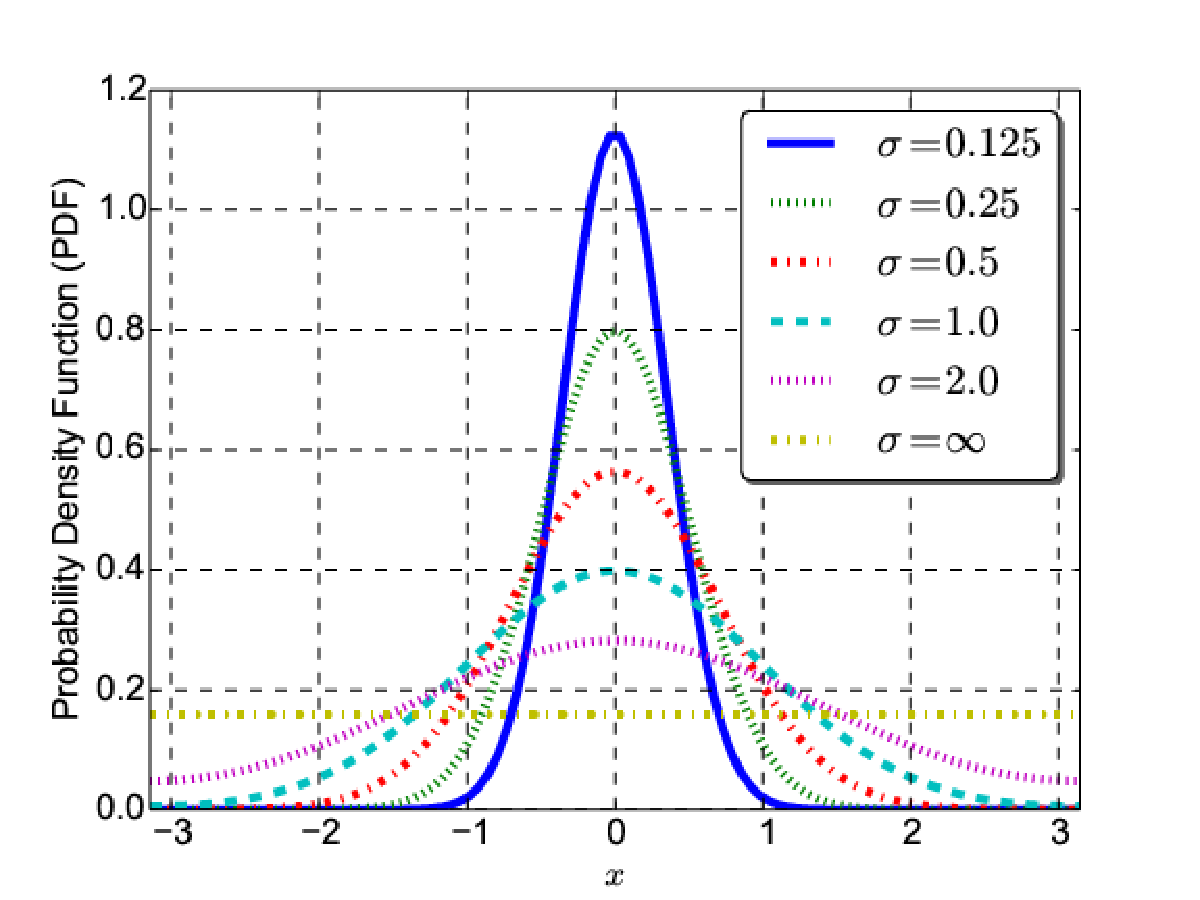
\includegraphics[width=80mm]{wrapped_gaussian_pdf}
  \caption{\label{fig:wrapped_gaussian_pdf} \emph{
    The probability density functions(PDFs) of the wrapped Gaussian
    distribution with different $\sigma_p$}.}
\end{figure}
%
%
%
After creating the spectrum distortion transfer function $D_l\left(e^{j(\omega_k)}\right)$
in \eqref{eq:spectrum_distortion}, we process each channel using the
structure shown in Fig. \label{eq:spectrum_distortion_block_diagram}.
We segment each microphone channels into successive frames with the
frame length of $160 ms$. The period between successive frames is $10 ms$.
We apply the Hanning window instead of the more frequently-used Hamming window
to each frame. We use the Hanning window to better satisfy the OverLap-Add (OLA)
constraint. After multiplying the complex spectrum of each frame with the
spectrum distortion transfer function $D_l\left(e^{j(\omega_k)}\right)$
in the frequency domain, the time-domain signal is re-synthesized
using OverLap-Add(OLA) synthesis. This processing is shown in detail
in Fig. \ref{fig:spectrum_distortion_block_diagram}. The reason for
going back to the time domain is because we use Complex Fast Fourier
Transform (CFFT) as feature whose frame size is $32 ms$ in Fig.
\ref{fig:entire_diagram}. 




%
%
\section{Experimental Results}
\label{sec:experimental_results}
%
\begin{table*}[th]
  \caption{\label{tab:result} {\it Speech recognition experimental result in terms of Word Error Rates (WERs).}}
  \vspace{2mm}
  \centerline{
    \begin{tabular}{| c | c | c | c | }
      \hline
                             & \specialcell{Baseline system \\ WER}  &  \specialcell{PDTR WER}  &   \specialcell{SDTR WER}  \\
      \hline \hline
      Original Test Set         &  11.87 \% & 12.07 \%  & 12.36 \%       \\
      \hline
      Simulated Noise Set       &  18.68 \% & 18.71 \%  & 19.40 \%       \\
      \hline
      \specialcell{Device 1  }  &  20.31 \% & 19.42 \%  & 19.57 \%      \\
      \hline
      \specialcell{Device 2  }  &  20.62 \% & 19.72 \%  & 19.64 \%      \\
      \hline
      \specialcell{Device 3  }  &  20.67 \% & 19.87 \%  & 20.17 \%     \\
      \hline
    \end{tabular}
  }
\end{table*}
%
In this section, we shows experimental results obtained with
the PDM and SDM. For training, we used an anonymized
22-million English utterances (15,000-hr), which are
hand-transcribed.  For training the acoustic model, instead of
directly using the these close-talking utterances, we use a
room simulator \cite{C_Kim_INTERSPEECH_2017_1} to generate
simulated utterances for our hardware.
In the simulator, we use 7.1 cm distance between two microphones.
For each utterance, one room configuration was selected out of
three million room configurations with varying room dimension, and
varying the target speaker and noise source locations. In each
room, number of noise sources may be up to three. This configuration
changes for each training utterance. Based on our experimental results,
after every epoch, we apply a different room configuration to the
utterance so that each utterance may be regenerated in somewhat
different ways.  For additive noise, we used Youtube videos,
recordings of daily activities, and recordings at various locations
inside cafes. We picked up the SNR value from a distribution
ranging from 0 dB to 30 dB, with an average of 11 dB. We used
reverberation time varying from 0 $ms$ up to 900.0 $ms$ with
an average of 500 $ms$. To model the reverberation, we employed
the image method \cite{J_Allen_JASA_1979}. We constructed
$17^3 - 1 = 4912$ virtual sources for each real sound source.
The acoustic model was trained using the Cross-Entropy (CE) minimization
as the objective function after aligning each utterance.

For evaluation, we used around 15-hour of utterances (13,795 utterances)
obtained from anonymized voice search data. Since our objective is
testing the robustness when our system is deployed in the actual hardware
we re-recorded these utterances using our actual hardware in a real room
at five different locations. We used three different devices as shown in
Table \ref{tab:result}. These three devices are prototype Google
Home devices. Each device is placed at five different positions and
orientations in a real room with mild reverberation. The entire
15-hour test utterances are rerecorded using each device.

In Table \ref{tab:result}, we compare the performance of
the baseline system, the PDTR system, and the SDTR system.
In case of the PDTR system, we use $\sigma_m = 0$ , and
 $\sigma_p = 0.1$ in \eqref{eq:random_variables}. In case of
 the SDTR system, we used $\sigma_m = 2.0$ and $\sigma_p = 0.1$
in \eqref{eq:random_variables}. These values are heuristically
selected from a few microphone transfer functions we observed.
From this table, we may observe
that PDTR and SDTR system may slightly harm the original
test set. However, we observe that they show better speech recognition
accuracy on real hardware, which is much more important.







\section{Conclusions}
In this paper, we described the PDTR algorithm to add phase distortion
to the training set to make  the trained phase-sensitive neural net
model robust against various distortion in signals. Our experimental
results show that the phase-sensitive neural-net trained with PDTR is
much more robust against real-world distortions.

\section{Acknowledgements}
The authors are thankful to Dr. Eunjoon Cho and Dr. Kean Chin for helpful
discussions. This research was supported by Google.

\newpage
%\eightpt
\bibliographystyle{IEEEtran}
\bibliography{../../common_bib_file/common_bib_file}

\end{document}
